\documentclass[11pt]{article}


\usepackage{fullpage}
\usepackage{graphicx}
\usepackage{amsmath}
\usepackage{amssymb}
\usepackage{amsthm}
\usepackage{fancyvrb}

\newcommand{\myname}{Mehshan Mustafa}

\newenvironment{theorem}[2][Theorem]{\begin{trivlist}
\item[\hskip \labelsep {\bfseries #1}\hskip \labelsep {\bfseries #2.}]}{\end{trivlist}}
\newenvironment{lemma}[2][Lemma]{\begin{trivlist}
\item[\hskip \labelsep {\bfseries #1}\hskip \labelsep {\bfseries #2.}]}{\end{trivlist}}
\newenvironment{exercise}[2][Exercise]{\begin{trivlist}
\item[\hskip \labelsep {\bfseries #1}\hskip \labelsep {\bfseries #2.}]}{\end{trivlist}}
\newenvironment{problem}[2][Problem]{\begin{trivlist}
\item[\hskip \labelsep {\bfseries #1}\hskip \labelsep {\bfseries #2.}]}{\end{trivlist}}
\newenvironment{question}[2][Question]{\begin{trivlist}
\item[\hskip \labelsep {\bfseries #1}\hskip \labelsep {\bfseries #2.}]}{\end{trivlist}}
\newenvironment{corollary}[2][Corollary]{\begin{trivlist}
\item[\hskip \labelsep {\bfseries #1}\hskip \labelsep {\bfseries #2.}]}{\end{trivlist}}
\newenvironment{solution}{\begin{proof}[Solution]}{\end{proof}}
\newenvironment{idea}[2][Proof Idea.]{\textit{#1} #2}



\parindent0in
\pagestyle{plain}
\thispagestyle{plain}

\newcommand{\dated}{\today}
\newcommand{\token}[1]{\langle \text{#1} \rangle}

\begin{document}

\textbf{Introduction to the Theory of
Computation}\hfill\textbf{\myname}\\[0.01in]
\textbf{Chapter 3: The Church-Turing Thesis}\hfill\textbf{\dated}\\
\smallskip\hrule\bigskip

\begin{problem}{3.9}
Let a $k$-PDA be a pushdown automaton that has $k$ stacks. Thus a $0$-PDA is an NFA and a $1$-PDA is a conventional PDA. You already know that $1$-PDAs are more powerful (recognize a larger class of languages) than $0$-PDAs.
\end{problem}

\begin{problem}[Part]{a}
Show that $2$-PDAs are more powerful than $1$-PDAs.
\end{problem}

\begin{proof}
A $2$-PDA can simulate any $1$-PDA by using only one of it's stacks. Therefore, $2$-PDAs can recognize all the languages that are recognized by $1$-PDAs. Additionally, we show that $2$-PDAs can also recognize more languages, which are not recognized by $1$-PDAs. For example, the language $A = \{a^nb^nc^n \ | \ n \geq 0 \}$. The language $A$ is not a context free language\footnote{Example 2.36, Chapter 2.}, but we can construct a $2$-PDA to recognize $A$ as follows:
\begin{enumerate}
\item Read and push $a$'s on both stacks until a $b$ is read.
\item Once a $b$ is read, match it with an $a$ by popping an $a$ from the first stack. Keep reading and matching any subsequent $b$'s. Reject if the number of $a$'s and $b$'s are not equal.
\item Next, match $c$'s with $a$'s on the second stack. Accept if the number of $a$'s and $c$'s are equal, reject otherwise.
\item In above steps, also make sure the input string is in $a^*b^*c^*$.
\end{enumerate}
\end{proof}

\begin{problem}[Part]{b}
Show that $3$-PDAs are not more powerful than $2$-PDAs.
\end{problem}

\begin{proof}
To show that $3$-PDAs are not more powerful than $2$-PDAs, we show how two stacks can be used to simulate a Turing machine tape.
\begin{enumerate}
\item Place the two stacks horizontally next to each other. The stack on the right grows to the right, whereas the stack on the left grows to the left.
\item Mark the end of stacks by pushing $\$$ on both stacks. For now, assume that the input symbols are available on the RHS stack, followed by the $\$$ symbol. Later we show how to load input string on the RHS stack.
\item The read/write head is always at the top of the RHS stack.
\item To read, pop from the RHS stack, and to write, push on the RHS stack.
\item To move right, pop a symbol from the RHS stack and push it to the LHS stack.
\item To move left, pop a symbol from the LHS stack and push it to the RHS stack.
\item While reading, if $\$$ is popped from the RHS, then this indicates the end of the tape. In this case, the input symbol is assumed to be the blank and the $\$$ is pushed back on the RHS stack. The written symbol is pushed on the LHS stack. 
\item While reading, if $\#$ is popped from the RHS, the this indicates that the head is at the left most position of the tape. In this case, push the $\#$ back on the LHS stack and read again.
\end{enumerate}
\begin{center}
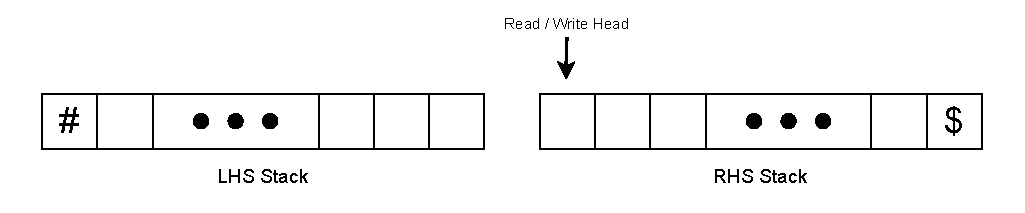
\includegraphics[scale=1.0]{Figures/Problem3.9.pdf} \\
Configuration of the two stacks. The RHS stack grows to the right, and the LHS stack grows to the left.
\end{center}
\end{proof}

\end{document}